%\documentclass[a4paper,12pt]{article}
\documentclass{book}
\usepackage[T1]{fontenc}
\usepackage [isolatin]{inputenc}
\usepackage{graphicx}
\usepackage{listings}

%\usepackage{fancyhdr}
%\pagestyle{fancy}
% with this we ensure that the chapter and section
% headings are in lowercase.
%\renewcommand{\chaptermark}[1]{%
%        \markboth{#1}{}}
%\renewcommand{\sectionmark}[1]{%
%        \markright{\thesection\ #1}}
%\fancyhf{} % delete current header and footer
%\fancyhead[LE,RO]{\bfseries\thepage}
%\fancyhead[LO]{\bfseries\rightmark}
%\fancyhead[RE]{\bfseries\leftmark}
%\renewcommand{\headrulewidth}{0.5pt}
%\renewcommand{\footrulewidth}{0pt}
%\addtolength{\headheight}{0.5pt} % space for the rule
%\fancypagestyle{plain}{%
%   \fancyhead{} % get rid of headers on plain pages
%   \renewcommand{\headrulewidth}{0pt} % and the line
%}

%\documentclass[a4paper,12pt]{book}
%\usepackage[T1]{fontenc}
%\usepackage [isolatin]{inputenc} % fontes avec caracteres accentues
%\usepackage{graphicx} % inclusion de figures
%\usepackage{listings}

\begin{document}

\title{\emph{NPTool 1.0 User Guide}}
\author{Adrien MATTA}

\maketitle 
\pagebreak
\tableofcontents % la table des matieres
\pagebreak

\chapter[NPTool]{NPTool}
\section {Introduction}

NPTool, Nuclear Physics Tool, aim to be a coherent set of programm usefull for Nuclear Physicist, especially those studying structure experimentally. 
Because each experiment is differents, people get used to exchange code and modified it to their needs. 
What NPT do is provinding an (try to be) universal framework so user can add their own functionnalities and share it with their collaborators. 
Geant4 and ROOT are now popular toolkit among the community, that's why NPTool use them widely and try to give a step by step process to use them efficiently.

In NPTool analysis and simulation are linked together. 
The proposed way of working is to generate an experiment like set of data and then annalysing with the future analysis code. 
Working this way help saving time by doing the biggest part of the analysis work in advance. 
It also help to understand what happen during analysis. 

				\begin{figure}[!htbp]
					\centering
					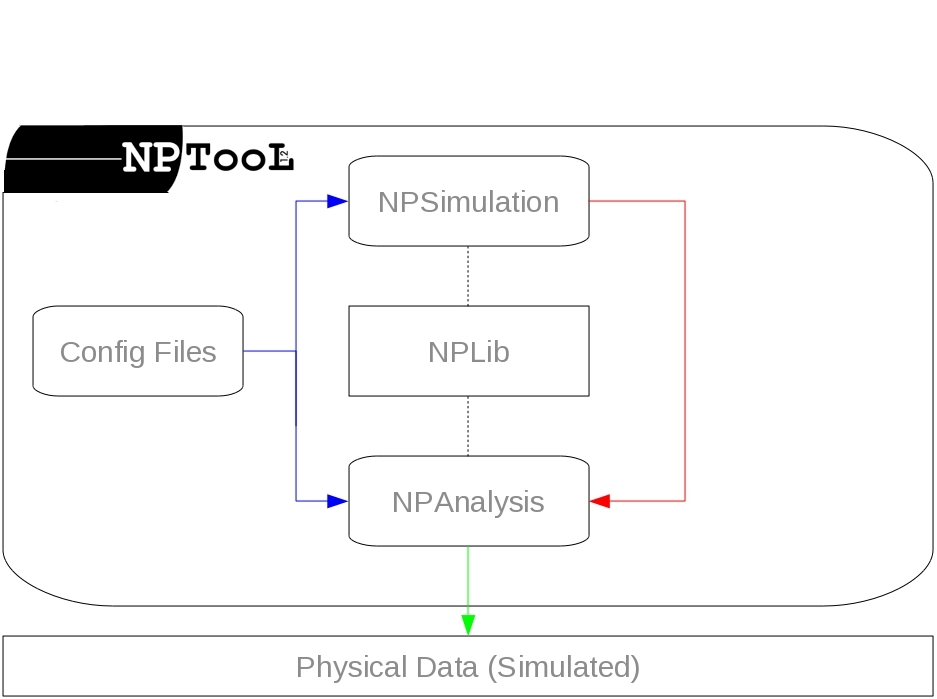
\includegraphics[width=0.5\textwidth]{./pictures/nptool_scheme_Sim.png}
					\caption{ \emph{Phase 1: Preparing an experiment} }
				\end{figure}

				\begin{figure}[!htbp]
					\centering
					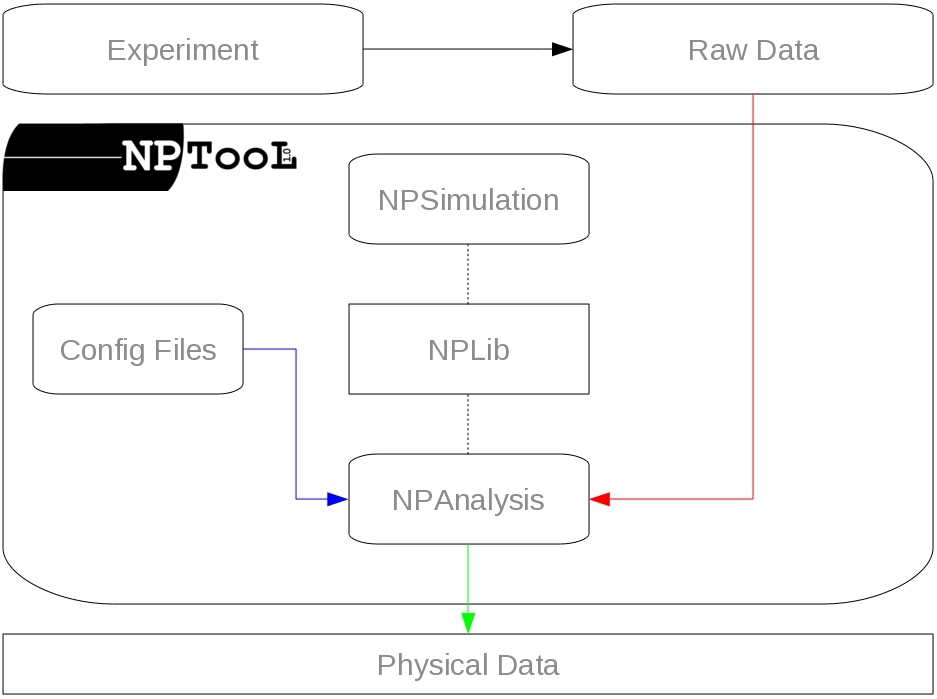
\includegraphics[width=0.5\textwidth]{./pictures/nptool_scheme_Ana.png}
					\caption{ \emph{Phase 2: Analysing an experiment} }
				\end{figure}	
				
				
				
\section{The directory layout}
	NPTool come with a specific directory layout. 
	The different make file and source are made to use this layout, using the environment variable. 
	Here is the standard layout:
		\begin{itemize}
			\item[-] NPLib : hold the libraries used both in NPA and NPS (NB: those librairies can be use in your own independant code if needed)
			\item[-] NPSimulation : hold the NPSimulation code
			\item[-] NPAnalysis: this folder contain one folder for each analysis project, feel free to make new one on the basis of the template one for instance
			\item[-] Inputs: this folder contain several folder, one for each type of intput, where you can find the input file used by the programm
			\item[-] Outputs: find here the outputs file of your simulation and analysis project
			\item[-] NPDocumentation: hold the documentation file
			\item[-] Licence: Take a look to the licence file and the list of contributor
			\item[-] \_MTN: you can some time find this folder, it not exactly part of the NPTool project, and is used only if you are working on the monotone data base (ie: if you are a contributor)
			\item[] 		
		\end{itemize}
%%%%%%%%%%%%%%%%%%%%%%%%%%%%%%%%%%%%%%%%%%%%%%%%%%%%%%%%%%%%%%%%%%%%%%%%
\chapter[NPLib]{NPLib}
	\section{Introduction}
	
	NPLib is the core package of NPTool, it contain several classes used in both analysis and simulation programm.
	NPTool versatility relly on this common core, its allow both programm to speak the same language in some way and also reduce drastically the amount of file since they are shared.
	NPLib is widely build on top of ROOT,GSL and CLHEP (by order of importance), but not on Geant4.
	
	\section{the directory layout}
		NPLib is made of several folder, one for each detector basicly and some for other shared object such as reaction and nucleus class. A common makefile is present in the NPLib directory calling the individual make file of every folder. In this folder you will also find a README file and the liblist file, containing a small macro used in NPA and NPS makefile to return the list of avaible librairies. Our phylosophy is to have two class for each detector, inheritted fron the TObject ROOT class so theyr can be put in a TTree. The first one is called the Data class, named following the TDetectorNameData, where T is there to remind the TObject dependance. This Data class hold the raw parameter given by the detector during an experiment, understood before any treatment. NPSimulation will output those kind of raw data, the only difference between a simulated and an experiement data object is the one comming from NPS are already calibrated. The second class is a Physics class, named TDetectorNamePhysics. This class hold the results of the treated Data object, ie after application of threshold, selection of good event, application of calibration,... and so one, depending on your detector. Note that the Physics class also derived from the VDetector class, and therefore can be used in NPA via the DetectorManager class. This system allow your annalysis programm to be more flexible and lisible. Let's have a look to the Directory layout:
		
		
		\begin{itemize}
			\item[DummyDetector] Template base for making your own Data and Physics class
			\item[AnnularS1] Containing the Data object for the Annular detector "S1" by micron 
			\item[GASPARD] Data and Physics object associate to the Gamma and Segmented Particule ARray Detector
			\item[MUST2] Data and Physics object associate to the MUr a STrip 2 detector
			\item[Plastic] Data and Physics object associate to the Plastic scintillator detector
			\item[SSSD] Data and Physics object associate to the Single Sided Striped Detector
			\item[InitialConditions] Used in NPS to output the initial physics condition of the generated event (Beam interaction position and energy, angle and energy of particule,...)
			\item[InteractionCoordinates] Used in NPS to output the true physical point of interaction in the differents detector
			\item[CalibrationManager] This class allowed to manage different file and token and associate them to detector
			\item[IORoot] Hold the ROOTInput and ROOTOutput classes that allow an easier used of TTRee in NPS and NPA
			\item[Tools] A few usefull classes such as Nuclear Reaction kinematics, Nucleus object and Energy Loss
			\item[VDetector] Virtual Detector class from wich inherrited all Physics class
			\item[include] All header are copy in this folder during compilation
			\item[lib] All libraries are copy in this folder during compilation
		\end{itemize}
		
	\section{Step by step from TDUMMYDetectorData class}
		\subsection{step 1}
			First, go to your consol and open the NPLib folder, there type \begin{verbatim}make distclean\end{verbatim}
			This command will remove all the compilation generated file and only the source will remain.
			Copy the DummyDetector folder and rename it, let's say, WonderdullDetector. 
			Ebter the directory and rename the TDummyDetectorData.h and .cxx with your detector name, you should have now only three file: Makefile, TWonderfullDetectorData.h and TWonderfullDetectorData.cxx
			If any other file remain, just remove it.
			No open the .h and .cxx file with your favorite editor (gedit or vim for instance). Replace the the DUMMYDetector by your detector name. Just have look in the .h file, the class is very basic, a couple of value are stored in stl vector (allowing smaller tree and increasing speed access). A few methods allowed to set or get those value and to know the size of the different vector. 
%%%%%%%%%%%%%%%%%%%%%%%%%%%%%%%%%%%%%%%%%%%%%%%%%%%%%%%%%%%%%%%%%%%%%%%%
				
\chapter[NPSimulation]{NPSimulation}

\section{Introduction}

NPSimulation is build on top of Geant4. 
It's provide a coherent and modular sets of classes that can be easily modified for your purpose.

\subsection{ The way it's work }

Because NPS is build on top of Geant4, you need C++ knowledge and Geant4 skills to understand how NPS work. 
NPS is a build as a modular basis that fit Nuclear Physicist needs: 
	\begin{itemize}
		\item Generate Nuclear Physics Event (such as a transfert, a beam, an ion source,... ) 
		\item Mange Detectors geometry (Number of module, positionning...)
	\end{itemize}
NPTool
NPS used two input files, one for the EventGenerator, and one for the Detectors Geometry. 
Those file are regroup in the \$NPT/Input directory wher you can find the EventGenerator and the DetectorConfiguration folder. 
If you want to add a new case you just have to create a new file in those directory. 
Note that files in the input directory are token readable file. It mean that they are not compile with the code, just read at each programm lauch. 
This way you can change the position of your detector or the energy of your beam for example without recompile the code. 
You can also quickly exchange your file with collaborators.

\section{ Running a simulation with existing detectors and event generator }

Running a NPSimulation is quite simple, first, start a console terminal (shell) and put your self in the NPS directory.
If you have add the environment variable correctly you can use the \emph{NPS} short cut that open the NPSimulation directory.
	
	\begin{verbatim}
			[myName@myDomain ~]$ NPS
			
			[myName@myDomain NPSimulation]$ Simulation myReaction myDetector
	\end{verbatim}
	
\emph{NB: order of arguments is essential. Both file need to be in the associated directory (see previous section).}

\emph{Simulation} is their a shortcut (or alias) added in the environment variable. 
In fact Geant4 generate the binari file in the path \$NPS/bin/YourSystem/ where "YourSystem" depend of you compilator and OS (for example \emph{Linux-g++}). 
Thats why we use a convinient shortcut.

After typing that command you will have a typical shell output of Geant4
\begin{verbatim}
*************************************************************
Geant4 version Name: geant4-09-01-patch-03 (12-September-2008)
                     Copyright : Geant4 Collaboration
                     Reference : NIM A 506 (2003), 250-303
                           WWW : http://cern.ch/geant4
*************************************************************
\end{verbatim}

Followed by the echo of what are in your input file. 
Check their that the token are well detected and everything correctly instantiate.

Then you have some standard Geant4 output again and the idle consol where you can tape any of the common Geant4 command, such as launching a run of 100 event:
\begin{verbatim}
Idle> run/beamOn 100
\end{verbatim}

If you want to display the tracking of particle in the differente volume and check the Energy loss you can type the following line. 
Keep in mind that display slow down the computation.

\begin{verbatim}
Idle> tracking/verbose 1
\end{verbatim}

The simulation will use the configured EventGenerator describe in your input file to generate events. 
Geant4 will deal with the particle tracking, energy loss, decay,... 
and the NPS framework generate an output ROOT file in the \$NPT/Output/Simulation directory. Default name for this file is mySimul.root. 
Since the file is regenerated at each execution, one need to rename it in order to keep it.

\section{ Adding a detector to NPS }

\subsection{ the VDetector class}

First you can have a look to the VDetector.hh file in the \$NPS/include directory. 
All the detector inherited from this Virtual class (V in VDetector stand for that, following the Geant4 naming convention). 
A virtual class described what should be the standard features of the inherited object. 
In this case their is 5 methods: Note thats those method are virtual, wich mean they are not implemented within this virtual class but in the daughter class. 
That allow to have the same method implemented differently for each detector. 
The " = 0 " following the class header mean that compilation failed if the daugter class do not have its own method definition (wich can be eventually empty).
A Vector of VDetector is manage by the DetectorConstruction file (see DetectorConstruction.hh and .cc) wich call those method automatically.

	\begin{itemize}
		\item[] ReadConfiguration(string): Read the file describing the Detector Configuration, ie: number of detector, position, and other option
		\item[] ConstructDetector(G4LogicalVolume*): Argument is the world volume. The method construct the volume
		\item[] ReadSensitive(const G4Event*): Read the scorer associate the to the sensitive method
	\end{itemize}
	
The two last methods are followed by a "{}" wich mean you are free to implemented or not. 
If not they will remain empty.
	\begin{itemize}
		\item[] InitializeRootOutput(): Instantiate a new Root Data object (see NPLib) and associate it to a new branch
		\item[] InitializeScorers(): Initialize the scorer (see GeneralScorer.hh and Geant4 Documentation)
	\end{itemize}

\section{ Step by Step from the DUMMYDetector class}
	The DUMMYDetector is a simple example of detector class manage in NPSimulation. 
	We will use this class as a starting point for adding your new detector

	\subsection{Step 1 : copying}
		An easy step, just copy the file DummyDetector.cc and DummyDetector.hh in the NPSimulation/src and NPSimulation/include directory. 
		Then rename them after your detector name, let say WonderfulDetector for the rest of the exemple. 
		Open them with your favorite editor and use the replace function to replace all the DUMMYDetector occurence by your detector name, WondenfulDetector. 
		You almost have finnish...

	\subsection{Step 2 : adding your detector to the Detector Construction}
		In order to allow the detector construction ton instantiate detector of yours you have to "tell him" to search for such detector. 
		Open the DetectorConstruction.cc file in the NPSimulation/src directory. 
		Have a look at the preprocessor includes, their is a list of all the detector avaible, just add a line with your file :
	\begin{verbatim}
	#include "WinderfulDetector.hh"
	\end{verbatim}

		Now DetectorConstruction know the WonderfulDetector class, but do not know how to find it in an input file. 
		Have look to the DetectorConstruction::ReadConfigurationFile method. 
		In this method Detector construction is reading the detector input file and looking for what kind of detector are presents. 
		Every time a new kind of detector is detected, a new array of this kind is instantiate and inialize via is own ReadConfiguration method. 
		For that, every class need an "array starting" token, wich should be different of the "module starting" token. 
		In our case we will choose "WonderfulArray" as an array starting token. 
		In order to avoid infinite loop of adding and adding the same detector again and again we need a boolean check, that simply check this kind of array is not already instantiate. 
		First, add one of this boolean, lets called it cWonderful, your code should look like that

	\begin{verbatim}
		/////////Checking Boolean////////////////////
		bool cMUST2           = false;
		bool cAddThinSi       = false;
		bool cGeneralTarget   = false;
		bool cGPDTracker      = false;	// Gaspard Tracker
		bool cS1              = false;
		bool cPlastic         = false;
		bool cDummy         	= false;
		bool cWonderful				= false;
	\end{verbatim}


	Then add the small searching sequence right after the Dummy Detector Sequence:
			
	\begin{verbatim}
					////////////////////////////////////////////
					/////// Search for a Dummy Detector ////////
					////////////////////////////////////////////
					else if (LineBuffer.compare(0, 16, "TheDUMMYDetector") == 0 && cDummy == false) {
						cDummy = true ;
						G4cout << "//////// DUMMY DETECTOR ////////" << G4endl << G4endl;

						// Instantiate the new array as a VDetector Object
						VDetector* myDetector = new DUMMYDetector();

						// Read Position of detector
						ConfigFile.close();
						myDetector->ReadConfiguration(Path);
						ConfigFile.open(Path.c_str());

						// Add array to the VDetector Vector
						AddDetector(myDetector);
					}

					////////////////////////////////////////////
					//// Search for a Wonderful Detector //////
					////////////////////////////////////////////
					else if (LineBuffer.compare(0, 15, "WonderfulArray") == 0 && cWonderful == false) {
						cWonderful = true ;
						G4cout << "//////// wonderful ARRAY ////////" << G4endl << G4endl;

						// Instantiate the new array as a VDetector Object
						VDetector* myDetector = new WonderfulDetector();

						// Read Position of detector
						ConfigFile.close();
						myDetector->ReadConfiguration(Path);
						ConfigFile.open(Path.c_str());

						// Add array to the VDetector Vector
						AddDetector(myDetector);
		      }
	\end{verbatim}

	\subsection{Step 3 : Data output}

	Lets have look to your Detector code. Open the WonderfulDetector.hh file and look at the private member, you should find the following line

	\begin{verbatim}
		////////////////////////////////////////////////////
		///////////Event class to store Data////////////////
		////////////////////////////////////////////////////
		private:
			TWonderfulDetectorData* m_Event ;

	\end{verbatim}

	The TWonderfulDetectorData class probably do not exist yet. 
	So you will have to create one, for that, follow the tutorial in the NPLib chapter. 
	If this class do not exist and you do not want to create one right now, simply use the TDUMMYDetectorData class instead (do not forget to change also the preprocessort include as well).

	\subsection{Step 4 : Token definition}
		NPS use input file with token detection. 
		For each detector there is at least two token, we already see one in the previous part, the array starting token. 
		You will need a second one, the module starting one, let choose "WonderfulModule". 
		So have a look at the WonderfulDetector::ReadCOnfiguration method. 
		In this method a loop over the config file is made, once the module starting bloc is fine, the ReadingStatus is set to true, wich mean we toggle to a module token search mode. 
		Generally speaking the "\%" simbole is used as a comment symbole and every caracter after this symbole will be skipped until the end of line. 
		This is the first token search. 
		Then come the search for another module starting search, here a security to avoid wrong token sequence. 
		Then come the list of all token. 
		You can add as many token as you need following the same model. 
		Just add one for exercise your self,

		\begin{description}
			\item[1:] Copying the THETA token bloc
			\item[2:] We want to add a Token associate to the number of stage in our detector. At the beginning of the function let create an integer name NumberOfStage and set it to 0. We also need a boolean to check the token as been found, just create a boolean named check\_NumberOfStage, and set it to false (have a look to the other variable such as Theta and check\_Theta).
			\item[3:] Change THETA to your new token, for instance "HOW\_MANY\_STAGE=" (note that token can't have space and always finnish by =). This new token have 15 caracter, so change the second argument of the compare method from 6 to 15.
			\item[4:] Change check\_Theta to check\_NumberOfStage and \emph{Theta = atof(DataBuffer.c\_str())} to \emph{NumberOfStage = atof(DataBuffer.c\_str())}. Remove the \emph{Theta=Theta*deg} and change the cout to display a corrected message.
		\end{description}

		
		\subsection{Step 5 : Material definition}

		Just have a look at the InitializeMaterial function. 
		You can here define as many as needed material after adding a private G4Material* object member to your classe. 
		Remember to delete those new object in the detector destructor. Those material can then be used in the volume definition. 
		This way each material are defined only one time per array, assuring a low number of material and therefor a low time running.

		\subsection{Step 6 : Scorer definition}
	
	Let's define a Scorer as class object allowing you to perform any kind of measurement.NPSimulation used G4VPScorer (see the G4 documentation for more detail), understand Virtual Primitive Scorer. 
	This virtual class allow Geant4 user to define the kind of scorer they want. 
	Initially scorer were design to allow user to monitor some physical value inside a logical volume without using the ReadSensitive class and ReadOutGeometry. 
	However, dure to their conception, those object was slow and running time quickly increased with the number of scorer... 
	In NPSimulation we improve this system, using a new way of indexing data in scorer and delete them when they are not needed anymore and the running time is acceptable. 
	Moreover, the Scorer simplify the code reading and allow user to come with their own set of scorer file dedicate to their detector. 
	We implement some General Purpose scorer that you can use as well.

%%%%%%%%%%%%%%%%%%%%%%%%%%%%%%%%%%%%%%%%%%%%%%%%%%%%%%%%%%%%%%%%%%%%%%%%
\chapter[NPAnalysis]{NPAnalysis}

\end{document}

